\documentclass{article}

\usepackage{amsmath, amsthm, amssymb, amsfonts}
\usepackage{thmtools}
\usepackage{graphicx}
\usepackage{setspace}
\usepackage{geometry}
\usepackage{float}
\usepackage{hyperref}
\usepackage[utf8]{inputenc}
\usepackage[english]{babel}
\usepackage{framed}
\usepackage[dvipsnames]{xcolor}
\usepackage{tcolorbox}

%Define the listing package
\usepackage{listings} %code highlighter
\usepackage{color} %use color
\definecolor{mygreen}{rgb}{0,0.6,0}
\definecolor{mygray}{rgb}{0.5,0.5,0.5}
\definecolor{mymauve}{rgb}{0.58,0,0.82}
 
%Customize a bit the look
\lstset{ %
backgroundcolor=\color{white}, % choose the background color; you must add \usepackage{color} or \usepackage{xcolor}
basicstyle=\footnotesize, % the size of the fonts that are used for the code
breakatwhitespace=false, % sets if automatic breaks should only happen at whitespace
breaklines=true, % sets automatic line breaking
captionpos=b, % sets the caption-position to bottom
commentstyle=\color{mygreen}, % comment style
deletekeywords={...}, % if you want to delete keywords from the given language
escapeinside={\%*}{*)}, % if you want to add LaTeX within your code
extendedchars=true, % lets you use non-ASCII characters; for 8-bits encodings only, does not work with UTF-8
frame=single, % adds a frame around the code
keepspaces=true, % keeps spaces in text, useful for keeping indentation of code (possibly needs columns=flexible)
keywordstyle=\color{blue}, % keyword style
% language=Octave, % the language of the code
morekeywords={*,...}, % if you want to add more keywords to the set
numbers=left, % where to put the line-numbers; possible values are (none, left, right)
numbersep=5pt, % how far the line-numbers are from the code
numberstyle=\tiny\color{mygray}, % the style that is used for the line-numbers
rulecolor=\color{black}, % if not set, the frame-color may be changed on line-breaks within not-black text (e.g. comments (green here))
showspaces=false, % show spaces everywhere adding particular underscores; it overrides 'showstringspaces'
showstringspaces=false, % underline spaces within strings only
showtabs=false, % show tabs within strings adding particular underscores
stepnumber=1, % the step between two line-numbers. If it's 1, each line will be numbered
stringstyle=\color{mymauve}, % string literal style
tabsize=2, % sets default tabsize to 2 spaces
title=\lstname % show the filename of files included with \lstinputlisting; also try caption instead of title
}
%END of listing package%
 
\definecolor{darkgray}{rgb}{.4,.4,.4}
\definecolor{purple}{rgb}{0.65, 0.12, 0.82}
 
%define Javascript language
\lstdefinelanguage{JavaScript}{
keywords={typeof, new, true, false, catch, function, return, null, catch, switch, var, if, in, while, do, else, case, break},
keywordstyle=\color{blue}\bfseries,
ndkeywords={class, export, boolean, throw, implements, import, this},
ndkeywordstyle=\color{darkgray}\bfseries,
identifierstyle=\color{black},
sensitive=false,
comment=[l]{//},
morecomment=[s]{/*}{*/},
commentstyle=\color{purple}\ttfamily,
stringstyle=\color{red}\ttfamily,
morestring=[b]',
morestring=[b]"
}
 
\lstset{
language=JavaScript,
extendedchars=true,
basicstyle=\footnotesize\ttfamily,
showstringspaces=false,
showspaces=false,
numbers=left,
numberstyle=\footnotesize,
numbersep=9pt,
tabsize=2,
breaklines=true,
showtabs=false,
captionpos=b
}

\colorlet{LightGray}{White!90!Periwinkle}
\colorlet{LightOrange}{Orange!15}
\colorlet{LightGreen}{Green!15}

\newcommand{\HRule}[1]{\rule{\linewidth}{#1}}

\NewEnviron{NORMAL}{% 
    \scalebox{2}{$\BODY$} 
} 

\declaretheoremstyle[name=Theorem,]{thmsty}
\declaretheorem[style=thmsty,numberwithin=section]{theorem}
\tcolorboxenvironment{theorem}{colback=LightGray}

\declaretheoremstyle[name=Proposition,]{prosty}
\declaretheorem[style=prosty,numberlike=theorem]{proposition}
\tcolorboxenvironment{proposition}{colback=LightOrange}

\declaretheoremstyle[name=Principle,]{prcpsty}
\declaretheorem[style=prcpsty,numberlike=theorem]{principle}
\tcolorboxenvironment{principle}{colback=LightGreen}

\setstretch{1.2}
\geometry{
    textheight=9in,
    textwidth=5.5in,
    top=1in,
    headheight=12pt,
    headsep=25pt,
    footskip=30pt
}

% ------------------------------------------------------------------------------

\begin{document}

% ------------------------------------------------------------------------------
% Cover Page and ToC
% ------------------------------------------------------------------------------

\title{ \normalsize \textsc{}
		\\ [2.0cm]
		\HRule{1.5pt} \\
		\LARGE \textbf{\uppercase{Calcolo Numerico}
		\HRule{2.0pt} \\ [0.6cm] \LARGE{Corso A} \vspace*{10\baselineskip}}
		}
        
\date{\text{Ultima Compilazione - }\today}
\author{\textbf{Autore} \\ 
		Giuseppe Acocella \\
		2024/25\\}

\maketitle
\newpage

\tableofcontents

\newpage

%\begin{figure}[htbp]
    %\center
    %\includegraphics[scale=0.4]{img/classiComplessita2.png}
%\end{figure}

\section{Introduzione}

I temi principali trattati in questi appunti saranno riguardanti i processi matematici che ci permettono di analizzare la conversione da continuo a discreto, per poter fornire questi dati ad una macchina finita. Spesso questi approcci vengono utilizzati anche quando la complessità di un determinato algoritmo è troppo elevata e di conseguenza si preferisce analizzare delle approssimazioni discrete.

\vspace*{15px}

\subsection{Fasi dell'Analisi Numerica}

Elenchiamo le fasi dell'Analisi Numerica:

\begin{enumerate}
    \item La prima fase è lo studio del \textbf{Mondo Reale} che osserviamo.
    \item Grazie all'osservazione del \textbf{Mondo Reale} generiamo un \textbf{Modello Matematico Continuo} in una seconda fase.
    \item La terza fase cerca di \textbf{discretizzare} il modello precedente in uno \textbf{discreto}. Questo genera un errore detto \textbf{errore analitico}.
    \item Si cerca un \textbf{Metodo di Risoluzione} al \textbf{Modello Matematico Discreto} durante una quarta fase. Questo genera un errore detto \textbf{errore inerente}, dato dalla rappresentazione discreta di qualcosa di continuo.
    \item L'ultima fase è quella della \textbf{Soluzione Approssimata} trovata dal 
    \newline \textbf{Metodo di Risoluzione} proposto. Questo produce un errore detto \textbf{errore algoritmico}.
\end{enumerate}

\vspace*{15px}

\subsection{Errore Inerente ed Errore di Approssimazione}

Consideriamo una $x$ continua, la sua rappresentazione su una macchina sarà $\overline{x}$. Definiamo dunque i due errori $\varepsilon_{IN}$ ed $\varepsilon_{x}$:

\vspace*{8px}

\begin{enumerate}
    \item \textbf{Errore Inerente} $(\varepsilon_{IN})$: Assumendo una funzione $f$:
    \[ \varepsilon_{IN} \: = \frac{f(\overline{x}) \: - \: f(x)}{f(x)} \]

\vspace*{8px}

    \item \textbf{Errore di Approssimazione} $(\varepsilon_{x})$: Assumendo una funzione $f$:
    \[ \varepsilon_{x} \: = \frac{\overline{x} \: - \: x}{x} \]
\end{enumerate}

\newpage

\subsection{Rappresentazione Virgola Fissa vs Virgola Mobile}

Immaginiamo di avere una quantità $k$ fissata di bit da poter utilizzare per rappresentare un numero su una macchina. Descriviamo due potenziali metodologie di rappresentazione:

\begin{enumerate}
    \item \textbf{Numeri a virgola fissa}: Si compongono di un \textbf{segno}, una \textbf{parte intera} ed una \textbf{parte frazionaria}.
    \item \textbf{Numeri a virgola mobile}: Si compongono di una \textbf{mantissa} ossia un numero compreso tra $0$ ed $1$ (estremi esclusi), un \textbf{segno} ed un \textbf{esponente}.
\end{enumerate}

\subsection{Teorema di Rappresentazione in Base}

Sia $x \in \mathbb{R}$, $x \neq 0$, allora scelta una base $\beta$ di rappresentazione \textbf{esistono} e \textbf{sono unici}:

\begin{enumerate}
    \item Un valore $\rho \in \mathbb{Z}$ detto \textbf{esponente}.
    \item Una successione $ \{ d_{i} \}_{i=1,2...}$ dette \textbf{cifre}.
    \item $d_{i}$ non tutte uguali a $\beta -1$ da un certo punto in poi.
\end{enumerate}

tali che:

\[ x \: = \: segno(x) \: \beta^{\rho} \: (\sum^{\infty}_{i=1} d_{i}\beta^{-i} ) \]

\subsubsection{Motivazioni e commenti}

\begin{enumerate}
    \item $d\neq0$ altrimenti avrei \textbf{rappresentazioni diverse} di \textbf{stessi numeri}, di conseguenza cadrebbe l'\textbf{unicità} delle rappresentazioni.
    \item $d_{i}$ non tutte uguali a $\beta -1$ da un certo punto in poi altrimenti numeri come $0.\overline{9}$ convergerebbe ad $1$.
\end{enumerate}

\vspace*{10px}

\subsection{Insieme di Numeri di Macchina}

Definiamo l'insieme $\Phi$ che permette la rappresentazione dei numeri di macchina:

\[ \Phi(\beta, t, m,M) = \: \{0\} \: \cup \: \{ x \in \mathbb{R} \: , x \: = \: segno(x) \: \beta^{\rho} \: (\sum^{t}_{i=1} d_{i}\beta^{-i} ) \} \]

\begin{enumerate}
    \item $\beta$: \textbf{base}.
    \item $t$ cifre della \textbf{mantissa}.
    \item $-n\leq \rho \leq M$, ossia i due \textbf{estremi} che contengono l'\textbf{esponente} $\rho$.
    \item Sono necessarie delle ipotesi a supporto dell'\textbf{unicità} di questa formulazione:
    \begin{enumerate}
        \item $0 \leq d_{i} \leq \beta-1$
        \item $d_{1} \neq 0$
    \end{enumerate}
\end{enumerate}

\newpage

\subsubsection{Cardinalità dell'Insieme di Numeri di Macchina}

\[ \# \Phi (\beta, t, m,M) = 1 \: + \: 2 (n+M+1)(\beta-1)(\beta^{t-1}) \]

\begin{enumerate}
    \item $1$ è la cardinalità dello \textbf{zero}.
    \item Il prodotto con $2$ è dato dal \textbf{segno}.
    \item $(n+M+1)$ tutte le possibili \textbf{configurazioni} dell'\textbf{esponente} $\rho$.
    \item $(\beta-1)$ tutte le possibili \textbf{configurazioni} delle \textbf{cifre} rispetto alla base (escluso lo zero).
    \item $(\beta^{t-1})$ avendo $t$ \textbf{bit disponibili} e $\beta$ la \textbf{base}, allora ho tutte le possibili \textbf{combinazioni} (escluse tutte quelle che iniziano con lo zero).
\end{enumerate}

\subsubsection{Numero più piccolo/più grande}

Analizziamo la rappresentazione del numero $\omega$ \textbf{più piccolo} e del numero $\Omega$ più grande.

\begin{enumerate}
    \item Numero \textbf{più piccolo} rappresentabile $\omega$:
    \[ \omega = \beta^{-m}(0.10...0)_{\beta} = (\beta^{-m})(\beta^{-1}) = \beta^{-m-1} \]
Questo perchè vogliamo la nostra base $\beta$ elevata al più piccolo estremo degli esponenti $-m$ moltiplicata alla più piccola mantissa nella base corrente.
    \item Numero \textbf{più grande} rappresentabile $\Omega$:
    \[ \Omega = \beta^{M}(0.[\beta-1][\beta-1][\beta-1]) = \beta^{M}(1-\beta^{-t}) \]
Questo perchè vogliamo la \textbf{base} $\beta$ elevata al più grande dei possibili esponenti $M$, ripetendo nella mantissa tutte le cifre più grandi permesse dalla base.
    
\end{enumerate}

\vspace*{10px}

\subsubsection{Standard IEEE}

Lo \textbf{Standard IEEE} può essere rappresentato come istanza di $\Phi$:

\[ Standard_{IEEE}\:=\:\Phi(2,53,1021,1024) \]

Contando $1$ bit per il segno e $11$ bit per l'esponente, $52$ bit vengono dedicati alla mantissa ed ad alcuni simboli speciali, come $NaN$ oppure $\infty$.

\vspace*{10px}

\paragraph{Underflow/Overflow} Una volta stabilito questo standard, se l'esponente $\rho$ esce \newline dall'intervallo $[-m,M]$, allora:

\begin{enumerate}
    \item Se $\rho > M$ allora è \textbf{overflow}, e ad esempio in Matlab questo comportamento viene approssimato ad $\infty$.
    \item Se $\rho < -m$ allora è \textbf{underflow}, e in Matlab questo comportamento viene approssimato a $0$.
\end{enumerate}

\newpage

\section{Studio dell'Errore}

\subsection{Troncamento/Arrotondamento}

Se $\rho \in [-m,M]$ allora possono succedere due cose:

\begin{enumerate}
    \item $x \in \mathbb{R}$ si rappresenta su $t$ cifre della mantissa disponibili.
    \item $x \in \mathbb{R}$ ha bisogno di più cifre rispetto a quelle fornite per la mantissa. In questo caso posso operare in due modi:
    \begin{enumerate}
        \item \textbf{Troncamento}: $x$ viene rappresentato con il numero di macchina subito prima. Quindi $x$ viene rappresentato con il numero di macchina $\tilde{x}$ che sia più grande rappresentabile con $|\tilde{x} |\leq |x|$.
        \item \textbf{Arrotondamento}: $x$ viene rappresentato con $\tilde{x}$ numero di macchina più vicino.
    \end{enumerate}
\end{enumerate}

\paragraph{Errore Assoluto/Relativo}

Definiamo due tipi di errore:

\begin{enumerate}
    \item \textbf{Errore Assoluto} $(\epsilon)$:
    \[ \epsilon = \tilde{x} - x \]
    \item \textbf{Errore Relativo} $(\epsilon_{x})$:
    \[ \epsilon_{x} = \frac{\tilde{x} - x}{x} \]
    
\end{enumerate}

\subsubsection{Teorema di Errore di Rappresentazione (con Dim.)}

Sia $x \in \mathbb{R}$, $x \neq 0$ e $\omega \leq |x| \leq \Omega$ allora:

\begin{enumerate}
    \item Identificando con $u$ la \textbf{precisione di macchina}:
    \[ |\epsilon_{x}| < u \]
    ed oltre a questo:
    \begin{enumerate}
        \item Operando con \textbf{troncamento}:
        \[ u \: = \: \beta^{1-t} \]
        \item Operando con \textbf{arrotondamento}:
        \[ u \: = \: \frac{1}{2}\beta^{1-t} \]
    \end{enumerate}
\end{enumerate}

\newpage

\paragraph{Dimostrazione}

\begin{enumerate}
    \item Rappresentazione in base: 
    \[ x \: = \: \beta^{\rho} \: (\sum^{\infty}_{i=1} d_{i}\beta^{-i}) \:\:\: \text{con} \:\:\: \rho \in [-m,M] \]
    \item Assumiamo di star considerando i numeri di macchina in troncamento, dunque cambia l'indice della sommatoria in $t$ cifre:
    \[ x \: = \: \beta^{\rho} \: (\sum^{t}_{i=1} d_{i}\beta^{-i}) \:\:\: \text{con} \:\:\: \rho \in [-m,M] \]
    \item ****
    \[ |\tilde{x} - x| < |b-a| \]
    \item ***
    \[ |x| \geq \beta^{\rho-1} \: = \: \beta^{\rho}(0.1)_{\beta} \]
    \item Dunque alla fine possiamo ricavare $\tilde{x}$ della nostra macchina:
    \[ \boxed{\tilde{x} \: = \: x(1+\epsilon_{x})} \]
\end{enumerate}

\newpage

\subsection{Operazioni di Macchina}

Assumendo $\tilde{x},\tilde{y}$ con $\tilde{x},\tilde{y} \in \Phi(10,t,5,5)$ ma con $\tilde{x}+\tilde{y} \notin \Phi(10,t,5,5)$, risulta necessario definire nuove operazioni, ossia delle \textbf{operazioni di macchina}:
\begin{enumerate}
    \item \textbf{Operazione Somma}: Prendiamo la versione in floating point dell'operazione somma originale:
        \[\tilde{x} \oplus \tilde{y} = fl(\tilde{x}+\tilde{y})\]
    e l'\textbf{errore} generato sarà:
    \vspace*{10px}
    \[ \epsilon = \frac{(\tilde{x} \oplus \tilde{y}) - (\tilde{x} + \tilde{y})}{(\tilde{x} + \tilde{y})} \]
    \vspace*{10px}
    Si associa quindi un operazione reale ad una approssimativa di macchina, quindi anche che
    \[ |\epsilon| < u \]
    \item \textbf{Operazione Differenza}: Allo stesso modo approcciamo la differenza, anch'essa produrrà un errore:
    \vspace*{10px}
    \[ \epsilon = \frac{(\tilde{x} \oplus \tilde{y}) - (x + y)}{(x + y)} \]
    \vspace*{10px}
\end{enumerate}

\subsubsection{Errore nella Somma e suo Relativo Ordine (con Dim.)}

Mostriamo per step questa dimostrazione:

\begin{enumerate}
    \item Definizione di $\tilde{x}$:
    \[ {\tilde{x} \: = \: x(1+\epsilon_{x})} \:\:\:,\:\:\: {\tilde{y} \: = \: y(1+\epsilon_{y})}\]
    \item Prendiamo in considerazione \textbf{solo} l'errore sull'\textbf{operazione somma}:
    \[ \tilde{x} \oplus \tilde{y} = (\tilde{x} + \tilde{y})(1+\epsilon)\]
    \item Sostituiamo le definizioni di $(1.)$ in $(2.)$:
    \[ \tilde{x} \oplus \tilde{y} = [x(1+\epsilon_{x}) + y(1+\epsilon_{y})](1+\epsilon) \]
    \newpage
    \item Svolgiamo i prodotti:
    \[ \tilde{x} \oplus \tilde{y} = (x+y) + x\epsilon_{x} + y\epsilon_{y} + (x+y)\epsilon + x\epsilon_{x}\epsilon + y\epsilon_{y}\epsilon \]
    \item Considerando il fatto che gli ultimi due operandi sono generati dal prodotto di due epsilon diversi, li ignoriamo effettuando un \textbf{approssimazione al prim'ordine}:
    \[ \tilde{x} \oplus \tilde{y} = (x+y) + x\epsilon_{x} + y\epsilon_{y} + (x+y)\epsilon \]
    \item Tornando alla definizione di $\epsilon_{TOT}$ dell'operazione somma:
    \[ \epsilon = \frac{(\tilde{x} \oplus \tilde{y}) - (x + y)}{(x + y)} \]
    \vspace*{10px}
    Effettuiamo sostituzione di $\tilde{x} \oplus \tilde{y}$ approssimati al prim'ordine:
    \[ \epsilon_{TOT} = \frac{[(x+y) + x\epsilon_{x} + y\epsilon_{y} + (x+y)\epsilon] - (x + y)}{(x + y)} \: = \]
    \[ = \frac{x}{x+y}\epsilon_{x} + \frac{y}{x+y}\epsilon_{y} + \epsilon \]
    \item Otteniamo dunque i primi due operandi che rappresentano l'\textbf{errore inerente}, ossia quello che si propaga dalle precedenti operazioni, e l'\textbf{errore algoritmico}, causato dalla corrente operazione:
    \[ \boxed{\epsilon_{TOT} = \frac{x}{x+y}\epsilon_{x} + \frac{y}{x+y}\epsilon_{y} + \epsilon} \]
    \item Rendendo generica la formula ottenuta definiamo dei \textbf{coefficienti di amplificazione}:
    \[ \boxed{ \epsilon_{TOT} = \epsilon_{OP} + C_{1}\epsilon_{TOT}^{(k)} + C_{2}\epsilon_{TOT}^{(s)} } \]
    Questa formula di $\epsilon_{TOT}$ si basa su una generica operazione
    \[ \boxed{z^{(i)} = z^{(k)} \: op \:z^{(k)}} \]
    
\end{enumerate}

\newpage

\subsubsection{Teorema di Errore di Calcolo Funzione Razionale (con Dim.)}

Calcolo dell'errore totale $\epsilon_{TOT}$:

\[ \boxed{\epsilon_{TOT} = \epsilon_{IN} + \epsilon_{ALG}} \]

dove:

\begin{enumerate}
    \item L'\textbf{Errore Inerente} dipende esclusivamente dal problema:
    \[ \boxed{\epsilon_{IN} = \frac{f(\tilde{x}) - f(x)}{f(x)}} \]
    \item L'\textbf{Errore Algoritmico} dipende dalla scelta della funzione scelta:
    \[ \boxed{\epsilon_{ALG} = \frac{g(\tilde{x}) - f(\tilde{x})}{f(x)}} \]
\end{enumerate}

\paragraph{Dimostrazione}

\begin{enumerate}
    \item Prendendo $\epsilon_{TOT}$ (inteso come somma di $\epsilon_{IN}$ e $\epsilon_{ALG}$) sommiamo e sottraiamo $f(\tilde{x})$:
    \[ \epsilon_{TOT} = \epsilon_{IN} + \epsilon_{ALG} =\]
    \[ = \: \frac{g(\tilde{x})-f(x)+f(\tilde{x})-f(\tilde{x})}{f(x)} \]
    \item Distribuisco in modo tale da poter ricavare l'\textbf{errore inerente} (secondo operando):
    \[ \epsilon_{TOT} = \frac{g(\tilde{x})-f(\tilde{x})}{f(x)} \: + \: \frac{f(\tilde{x})-f(x)}{f(x)}  \]
    \item Moltiplico e divido per $f(\tilde{x})$ e scambio tra loro i due denominatori:
    \[ \epsilon_{TOT} = \frac{g(\tilde{x})-f(\tilde{x})}{f(\tilde{x})} \: * \: \frac{f(\tilde{x})}{f(x)}\:+\:\epsilon_{IN}  \]
    \item Notiamo che il primo fattore del primo operando corrisponde all'errore algoritmico:
    \[ \epsilon_{TOT} = \epsilon_{ALG} \: * \: \frac{f(\tilde{x})}{f(x)}\:+\:\epsilon_{IN}  \]
    \item Assumendo che $\epsilon_{IN+1} = \frac{f(\tilde{x})}{f(x)}$ sostituiamo:
    \[ \epsilon_{TOT} = (\epsilon_{ALG})(\epsilon_{IN+1})\:+\:\epsilon_{IN}  \]
    \item Approssimiamo $\epsilon_{ALG} \doteq (\epsilon_{ALG})(\epsilon_{IN+1})$:
    \[ \boxed{\epsilon_{TOT} = \epsilon_{IN} + \epsilon_{ALG}} \]
    
\end{enumerate}

\newpage

\subsubsection{Condizionamento vs Stabilità}

Descriviamo le differenze tra \textbf{condizionamento} e \textbf{stabilità}:

\begin{enumerate}
    \item \textbf{Condizionamento}: Studio dell'errore, errore intrinseco.
    \item \textbf{Stabilità}: Studio dell'errore algoritmico, rappresenta la stabilità
    \newline
    numerica dell'algoritmo proposto.
\end{enumerate}

\subsubsection{Teorema Coefficiente di Amplificazione ed Errore Inerente (con Dim.)}

Sia $f(x) \in C^{2}$ (ossia derivabili due volte con entrambe le derivate continue), allora:

\[ \boxed{\epsilon_{IN} = \frac{x}{f(x)}f^{'}(x)\epsilon_{x}} \]

Grazie a questo possiamo determinare se un problema risulta mal condizionato o ben condizionato:

\[ \boxed{C_{amplificazione} = \frac{x}{f(x)}} \]

\vspace*{5px}

\begin{enumerate}
    \item \textbf{Ben Condizionato}: Non ho punti nel dominio del coefficiente di amplificazione dove la funzione va a $\infty$.
    \item \textbf{Mal Condizionato}: Ho dei punti in cui il coefficiente può andare a $\infty$. Dunque un problema può essere mal condizionato in specifici intervalli.
\end{enumerate}

\paragraph{Dimostrazione}

\begin{enumerate}
    \item Riprendiamo lo sviluppo di Taylor fino al secondo ordine:
    \[ f(x) = f(x_0) + f^{'}(x_0)(x-x_0) + f^{''}(x_0)\frac{(x-x_0)^{2}}{2!}\]
    \vspace*{8px}
    \item Contestualizziamo ad $\tilde{x}$:
    \[ f(\tilde{x}) = f(x) + f^{'}(x)(\tilde{x}-x) + f^{''}(x)\frac{(\tilde{x}-x)^{2}}{2!}\]
    \vspace*{8px}
    \item Porto a sinistra $f(x)$:
    \[ f(\tilde{x}) -f(x) = f^{'}(x)(\tilde{x}-x) + f^{''}(x)\frac{(\tilde{x}-x)^{2}}{2!}\]
    \newpage
    \item Moltiplico e divido per $x$ il primo operando a sinistra e moltiplico e divido per $x^{2}$ il secondo operando a sinistra:
    \[ f(\tilde{x}) -f(x) = xf^{'}(x)\frac{(\tilde{x}-x)}{x} + x^{2}\frac{f^{''}(x)\frac{(\tilde{x}-x)^{2}}{2!}}{x^{2}}\]
    \item Considerando che:
    \begin{enumerate}
        \item Errore $\epsilon_{x}$ ed $\epsilon^{2}_{x}$:
        \vspace*{5px}
        \[ \boxed{\epsilon_{x} = \frac{(\tilde{x}-x)}{x}} \:\:\: \boxed{\epsilon^{2}_{x} = \frac{(\tilde{x}-x)^{2}}{x^2}} \]
    \end{enumerate}
    \vspace*{8px}
    \item Sostituiamo con $\epsilon_{x}$ ed approssimiamo al prim'ordine ignorando $\epsilon^{2}_{x}$:
    \[ f(\tilde{x}) - f(x) = xf^{'}(x)\epsilon_{x} \]
    \vspace*{8px}
    \item Dunque infine otteniamo la formula generica:
    \[ \boxed{\epsilon_{IN} = \sum_{i=1}^{n} \frac{x_{i}}{f(x_{1},...,x_{n})} \frac{\delta f}{\delta x_{i}} \epsilon_{x_{i}}} \]
\end{enumerate}

\vspace*{15px}

\subsubsection{Errore di Calcolo Funzione Irrazionale}

Assumiamo di voler rappresentare in macchina $e^x$. E' necessario trovare una funzione che approssimi la funzione irrazionale $e^x$:

\begin{enumerate}
    \item Definiamo $e^x$ ed $EXP(x)$:
    \[ \boxed{e^{x} = \sum^{\infty}_{i=0} \frac{x^{i}}{i!}} \: \: \: \: \: \: \: \: \boxed{EXP(x) = \sum^{n}_{i=0} \frac{x^{i}}{i!}} \]
    \item Valutiamo quanto intercorre tra le due con l'errore di \textbf{Lagrange}:
    \[ e^x = EXP(x) + \frac{\epsilon^{(n+1)}_{x}}{(n+1)!} \]
\end{enumerate}

In questo modo abbiamo stabilito che errore viene effettuato approssimando $e^x$ con $EXP(x)$.

\newpage

\section{Algebra Lineare Numerica - Computazione e Condizionamento}

Questo capitolo analizzerà strumenti base dell'algebra lineare che successivamente saranno richiesti per problemi su spazi vettoriali.

\subsection{Norme Vettoriali}

La norma è una \textbf{funzione} che ci permette di ricavare un informazione quantitativa dato un oggetto di uno specifico spazio vettoriale.

\paragraph{Definizione} Sia $f: F^{n} \xrightarrow{} \mathbb{R}$ tale che:

\begin{enumerate}
    \item $f(x) \geq 0 $ e $f(x) = 0$ se e solo se $x = \begin{bmatrix}
0 \\
. \\
. \\
0
\end{bmatrix}$

    \item $f(\alpha x) \: = \: |\alpha|f(x) \: \: \: \forall \alpha \in F $
    \item $f(x+y) \leq f(x) + f(y)$
\end{enumerate}

Allora $f$ è una norma vettoriale su $F$ e si definisce con $\boxed{|| \:\:\:||}$

\subsubsection{Distanza, Norma 1, Norma 2, Norma Infinito}

Elenchiamo queste definizioni:

\begin{enumerate}
    \item \textbf{Distanza}:
    \[ d(x,y) = || \: x - y \:|| \]
    \item \textbf{Norma 1}:
    \vspace*{8px}
    \[ || x ||_{1} = \sqrt{\sum^{n}_{i=1}}|x_{i}| \]
    \vspace*{4px}
    \item \textbf{Norma 2}:
    \vspace*{8px}
    \[ || x ||_{2} = \sqrt{\sum^{n}_{i=1}}|x_{i}|^2 \]
    \vspace*{4px}
    \item \textbf{Norma Inf*}:
    \vspace*{8px}
    \[ || x ||_{\infty} = nax|x| \]
    \vspace*{4px}
\end{enumerate}

\newpage

\paragraph{Equivalenza Topologica} Date due norme $||\:||_{(1)}$ e $||\:||_{(2)}$ allora $\exists \: \alpha,\beta \in F$ tale che $\forall \: v \in F^{n}$:
\[ \alpha||v||_{(2)} \leq ||v|| \leq \beta||v||_{(1)}\]

Da questo posso ottenere informazioni riguardo divergenza e convergenza se utilizzato "simil th. dei carabinieri".

\subsection{Norma Matriciale}

Contestualizziamo la norma alle matrici:

\paragraph{Definizione} Sia $f: F^{nxn} \xrightarrow{} \mathbb{R}$ tale che:

\begin{enumerate}
    \item $f(A) \geq 0$ e $f(A) = 0$ se e solo se $A = [0]_{nxn}$
    \item $f(\alpha A) = |\alpha|f(A)$
    \item $f(A+B) = f(A) + f(B)$
    \item $f(AB) \leq f(A)f(B)$
\end{enumerate}

\subsubsection{Norma Matriciale indotta da Norma Vettoriale}

% spiegazione e contesto

***********

\[||A|| \: = \: max||Av|| \: \: \: \: \textbf{con} \: \: \: \: ||v|| = 1\] 

\subsubsection{Norma di Frobanius}

************

% spiegazione e contesto

\[ ||A||_{F} = \sqrt{\sum^{n}_{i,j=1}|a_{ij}|^2} \]

\[ ||A||_{F} = traccia(A^{H}A)\footnotemark \]

\footnotetext{La traccia in una matrice corrisponde alla somma degli elementi sulla diagonale principale. La matrice indicata con H è la trasposta coniugata, ossia matrice su cui abbiamo eseguito rispettivamente l'inversione tra righe e colonne e invertito i segni alle componenti immaginarie.}

\newpage

\subsubsection{Th. Compatibilità delle Norme (con Dim*.)}

\begin{enumerate}
    \item Il teorema afferma questo:
    \vspace*{10px}
    \[ \boxed{||Ax|| \leq ||A||\:\:||x||} \]
\end{enumerate}

\paragraph{Dimostrazione} Dimostriamo il teorema:

\begin{enumerate}
    \item \textbf{Vettore Nullo}:
    \[ x=0 \Rightarrow vera \: , \: \: 0 \leq ||A|| * 0 \]
    \item \textbf{Vettore Strettamente Positivo}:
    \begin{enumerate}
        \item Prendo vettore $x$ e lo normalizzo:
        \[ \frac{x}{||x||} \]
        \item Prendo la norma del risultato e la pongo uguale alla norma di un ipotetico $y$:
        \[ ||y|| = ||\frac{x}{||x||}|| = \frac{1}{||x||} * ||x|| = 1 \]
        \item Seguendo la catena di uguaglianze precedenti ricaviamo:
        \[ ||\frac{x}{||x||}|| = 1 \]
        % non si capisce come continuare
        \item ******
    \end{enumerate}
\end{enumerate}

\subsubsection{Metodi Iterativi su Norme}

Elenchiamo le caratteristiche del calcolo iterativo delle norme:

\begin{enumerate}
    \item \textbf{Norma 1}: Somma delle \textbf{colonne}, ottengo un vettore, da questo prendo il massimo:
    \[ \boxed{||A||_{1} = max\sum^{n}_{i=1}|a_{ij}| \: \: \: \text{con} \: \: \: a_{ij} \in A}\]
    \item \textbf{Norma Infinito}: Somma delle \textbf{righe}, ottengo un vettore, da questo prendo il massimo:
    \[ \boxed{||A||_{\infty} = max\sum^{n}_{j=1}|a_{ij}| \: \: \: \text{con} \: \: \: a_{ij} \in A}\]
    \item \textbf{Norma 2}: Assumendo $\varphi$ sia raggio spettrale della matrice in questione, dove: \[\varphi(A) = max_{i=1...n} \: \:|\lambda_{i}|\]
    \vspace*{3px}
    \[ \boxed{||A||_{2} = \sqrt{\varphi(A^{H}A)}} \]
\end{enumerate}

\newpage

\subsubsection{Matrici Simmetriche sui Reali}

Elenchiamo proprietà caratterizzanti delle matrici simmetriche che verranno citate successivamente:

\begin{enumerate}
    \item $A = A^T$
    \item Le matrici simmetriche sui reali:
    \begin{enumerate}
        \item Sono \textbf{diagonalizzabili}
        \item Hanno \textbf{autovalori reali}
    \item $(A^TA)^T = (A\:A^T)$
    \item $||A||_2 = \varphi(A)$
    \end{enumerate}
\end{enumerate}

\subsubsection{Th. di Hirch (con Dim.)}

\paragraph{Definizione} Se $||\: .\:||$ è una norma matriciale indotta, allora:

\[ \lambda^{(A)} \: < \:||A|| \]


\begin{figure}[htbp]
    \center
    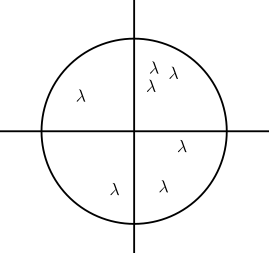
\includegraphics[scale=0.55]{img/th_hirch.png}
\end{figure}

Ossia ogni autovalore deve essere inferiore alla norma matriciale indotta.
E' come se stessimo "localizzando" la posizione degli autovalori.

\paragraph{Dimostrazione} Dimostriamo il teorema:

\begin{enumerate}
    \item Dalla definizione di autovalore:
    \[ A\:v = \lambda\:v \:\:\: \text{con} \:\:\: \lambda \neq0\]
    \item Applico la norma a sx e dx ed inverto l'ordine:
    \[ ||\:\lambda\:v\:|| = ||\:A\:v\:||\]
    \item Proprietà $(2.)$ e $(4.)$ delle norme matriciali:
    \[ \lambda\:||A|| = ||A\:v|| \leq ||A|| \:|| v || \]
    \item Considero dunque primo e terzo termine, dividendo a sx e dx per $||v||$:
    \[ \boxed{\lambda \leq ||A||} \]
\end{enumerate}

\newpage

\subsection{Utilities Greshgorin}

Elenchiamo tutte gli oggetti e funzioni definiti sui cerchi di Gershgorin:

\subsubsection{Cerchio i-esimo di Greshgorin}

Definiamo un cerchio come luogo geometrico dei punti, dato che successivamente sarà necessario alla localizzazione degli autovalori.

\paragraph{Definizione} Sia $K_{i}$ dove
\[ \boxed{K_{i} = \{ z \in \mathbb{C} \: : \: |z-a_{ii}| \leq \sum_{j=1, j\neq i}^{n}|a_{ij}|  \: \} }\]

\begin{enumerate}
    \item $a_{ii}$ corrisponde al \textbf{centro} del cerchio.
    \item $\sum_{j=1, j\neq i}^{n}|a_{ij}|$ corrisponde al \textbf{raggio} del cerchio.
\end{enumerate}

\subsubsection{Th. di Greshgorin (con Dim.)}

Il teorema di Greshgorin afferma che se un arbitrario $\lambda$ è un autovalore, allora questo deve essere all'interno dell'unione dei cerchi di Greshgorin della matrice.

\paragraph{Definizione} $\boxed{\text{Se} \: \: \: \lambda \: \: \: \text{è} \: \: \: \textbf{autovalore} \: \: \: \text{di} \: \: \: A \: \:\Rightarrow \: \: \lambda \in \bigcup_{i=1}^{n}k_{i}} $

\vspace*{12px}

Spesso questo teorema viene utilizzato "al contrario", ossia se un valore \textbf{non} è all'interno dell'unione dei cerchi, allora sicuramente \textbf{non} è un autovalore della matrice.

\paragraph{Dimostrazione} Dimostriamo il teorema:

\begin{enumerate}
    \item Dalla definizione di autovalore:
    \[ A\:v = \lambda \: v \]
   \[ \begin{bmatrix}
    a_{11} & a_{12} & ... & a_{1n}\\
    a_{21} & a_{22} & ... & a_{2n}\\
    . & . & . & . \\
    a_{n1} & a_{n2} & ... & a_{nn}
    \end{bmatrix} 
    \begin{bmatrix}
        v_1 \\
        v_2 \\
        . \\
        v_n \\
    \end{bmatrix} \: = \: \lambda 
    \begin{bmatrix}
        v_1 \\
        v_2 \\
        . \\
        v_n \\
    \end{bmatrix} \]
    \vspace*{5px}
    \item Assumo di aver effettuato il prodotto ad sx tra $A$ e $v$:
    \[ \sum_{j=1}^{n} a_{ij}v_{j} = \lambda v_{i} \:\:\:\: \forall \: i \in \{ 1\:,... ,\:n \}  \]
    \item Tiro fuori dalla sommatoria il termine per $i=j$, lo porto a sinistra e metto in evidenza $v_{i}$:
    \[ \sum_{j=1,j\neq i}^{n} (a_{ij}v_{j})  = (\lambda - a_{ii} )v_{i} \]
    \newpage
    \item Sapendo che:
    \[ \boxed{|\lambda-a_{ii}|\:|v_{i}|  =  | (\lambda - a_{ii})v_{i} |} \:\:\: \text{e} \:\:\: \boxed{|\sum_{j=1}^{n} a_{ij}v_{j} \:  | \leq \sum_{j=1}^{n} \:|a_{ij}|\:|v_{j}|} \]
    \item Prendo un $p$ tale che:
    \[ 0 \leq |v\:p| = ||v|| = max_{j=1..n} \: |v_{j}| \]
    Ossia $p$ deve fare in modo che la norma di $v$ deve essere uguale al massimo delle componenti del vettore $v$. Assumiamo di non star lavorando sul vettore nullo grazie alla definizione di autovalore $\lambda$.
    \item Istanzio il punto $(3.)$ con la $p$ appena definita in $(5.)$:
    \[ |\lambda - a_{pp }|  |v_{p}| \leq \sum_{j=1,j \neq i}^{n} |a_{pj}| |v_{j}| \]
    \item Divido a sx e dx per $|v_{p}|$:
    \[ |\lambda - a_{pp }|  \frac{|v_{p}|}{|v_{p}|} \leq \sum_{j=1,j \neq i}^{n} |a_{pj}| \frac{|v_{j}|}{|v_{p}|} \]
    Sappiamo che $\frac{|v_{j}|}{|v_{p}|} \leq 1$ perchè in un vettore possiamo avere più massimi, quindi componenti max con stessi valori.
    \item Riesco dunque ad effettuare una maggiorazione grazie alle affermazioni precedenti:
    \[ \sum_{j=1,j \neq i}^{n} |a_{pj}| \frac{|v_{j}|}{|v_{p}|} \leq \sum_{j=1,j \neq i}^{n} |a_{pj}| \]
    \item La sommatoria ottenuta nella maggiorazione del punto $(8.)$ rispetta la definizione di \textit{Cerchio i-esimo di Gershgorin}, di conseguenza abbiamo dimostrato il teorema. $\boxed{}$
    \[ \boxed{\lambda \in K_{p}} \]
    
\end{enumerate}

\subsubsection{Invertibilità e Predominanza Diagonale}

\paragraph{Matrice Invertibile} Elenchiamo un paio di caratteristiche sull'invertibilità di matrici:

\begin{enumerate}
    \item Se $A$ è invertibile, allora:
    \begin{enumerate}
        \item $det(A) \neq 0 $
        \item $rango(A) = 0$
        \item $dim(ker(A)) = 0$
        \item $0$ non è un autovalore
        \item $P(x) = det(A-xI) = (x-\lambda_{1})(x-\lambda_{2})....(x-\lambda_{n})$
        \item $P(0) = det(A) = (x-\lambda_{1})(x-\lambda_{2})....(x-\lambda_{n}) = \text{ prodotto degli autovalori }\lambda_{i}$
    \end{enumerate}
\end{enumerate}

\paragraph{Predominanza Diagonale di Matrice per Riga} La predominanza vale quando in valore assoluto, l'elemento sulla diagonale principale è maggiore di tutti gli altri sulla riga, formalmente:

\[ |a_{ii}| > \sum_{j=1,j \neq i}^{n}|a_{ij}| \]

\subparagraph{Corollario} Se $A$ è a \textbf{predominanza diagonale} allora $A$ è \textbf{invertibile}. La dimostrazione di questo corollario si basa sul fatto che la definizione appena data si basa sul \textit{Cerchio di Gershgorin} ma utilizzato al contrario, ossia stiamo affermando di \textbf{non} essere nel cerchio. Questo però ci porta ad essere esattamente al contrario rispetto ****.

\subsubsection{II Th. di Gershgorin}

\paragraph{Definizione} Se l'\textbf{unione} $M_{1}$ di $k$ cerchi è \textbf{disgiunta} dall'\textbf{unione} $M_{2}$ di $(n-k)$ cerchi allora $k$ autovalori appartengono ad $M_{1}$ ed $(n-k)$ ad $M_{2}$.

\subsection{Condizionamento del Problema sulla Risoluzione di Sistemi Lineari}

Assumiamo di avere una matrice $A$ ed un vettore $b$, $Ax = b$, sapendo che se $A$ è invertibile allora $x = A^{-1}b$, altrimenti o non ha soluzioni o ne ha infinite. Elenchiamo come approssimeremo questi oggetti in oggetti discreti:

\begin{enumerate}
    \item \textbf{Matrice} $A$ ed i suoi \textbf{elementi} $a_{ij}\:$:
    \[ \tilde{A} = A + \Delta A  \:\:\: \:\:\: \:\:\: \tilde{a}_{ij} = a_{ij} + \epsilon  f_{ij}  \]
    dove $f_{ij} = (1+\epsilon_{ij})$, ossia l'errore su ogni componente, e $\Delta A$ li contiene tutti.
    \item \textbf{Vettore} $b$ ed i suoi \textbf{elementi} $b_{i}\:$:
    \[ \tilde{b} = b + \delta b  \:\:\: \:\:\: \:\:\: \tilde{b}_{i} = b_{i} + (1+f_{i})  \]
\end{enumerate}

Il \textbf{condizionamento} verrà quindi calcolato su \textbf{norme}:

\[ \frac{||\tilde{x}-x||}{||x||} \]

Vogliamo dunque esprimere la risoluzione in questa forma:

\[ x = A^{-1}b \]

\subsubsection{Teorema* (con dim*)} 

\paragraph{Definizione} Sia $A$ invertibile e $b \neq 0$, allora:

\[ \frac{||\tilde{x}-x||}{||x||} \leq ||A||\:\:||A^{-1}|| \frac{||\tilde{b}-b||}{||b||} \]

Dove $||A||\:\:||A^{-1}||$ è detto \textbf{numero di condizionamento} di A.

\newpage

\paragraph{Dimostrazione} Dimostriamo questo teorema:

\begin{enumerate}
    \item Partiamo dalla definizione di $x$ ed $\tilde{x}$:
    \[ x = A^{-1}b \: \:\rightarrow \: \: Ax = b\]
    \[ \tilde{x} = A^{-1}\tilde{b} \: \:\rightarrow \: \: A\tilde{x} = \tilde{b}\]
    \item Sostituiamo $(1.)$ in $||\tilde{x}-x||$:
    \[ || \: A^{-1}\tilde{b} \: - \: A^{-1}{b} \: || \]
    \item Raccolta di $A^{-1}$ e compatibilità di norme a motivazione del $(\leq)$:
    \[ ||A^{-1}(\tilde{b}-b)|| \leq ||A^{-1}|| \: \: ||\tilde{b}-b|| \]
    \item Scriviamo la forma standard di risoluzione di sistema lineare applicando le norme a sx e dx, e utilizziamo anche qui la compatibilità delle norme per $(\leq)$ a dx:
    \[ ||Ax|| = ||b|| \: \rightarrow \: ||b|| = ||Ax|| \leq ||A|| \: \: ||x|| \]
\end{enumerate}

\newpage

\section{Metodi Diretti per Risoluzione di Sistemi Lineari}

Assumiamo di avere $Ax = b, \: \: \: A\in \mathbb{R}^{nxn}, \: \: \: det(A)\neq0, \: \: \: x = A^{-1}b$, allora possiamo avere diversi casi:

\begin{enumerate}
    \item \textbf{Matrice Diagonale}: La matrice $A$ ha solo elementi sulla sua diagonale.
    \[ 
    \begin{bmatrix}
    a_{11} & 0 & ...  & 0\\
    0 & a_{22} &  & ...\\
     ...&  & a_{33} &  0\\
     0& ... & 0 & a_{nn}
    \end{bmatrix} 
    \]
    In questo caso possiamo ricavare le \textbf{soluzioni} in questo modo
    \[ x = A^{-1}b = \begin{bmatrix}
    \frac{1}{a_{11}} & 0 & ...  & 0\\
    0 & \frac{1}{a_{22}} &  & ...\\
     ...&  & \frac{1}{a_{33}} &  0\\
     0& ... & 0 & \frac{1}{a_{nn}}
    \end{bmatrix}
    \begin{bmatrix}
    b_{1}\\    
    b_{2}\\
    b_{3}\\
    b_{n}
    \end{bmatrix}  \]
    Ricordiamo che il costo di questa risoluzione risulta essere $O(n)$.
    \item \textbf{Matrice Triangolare}: La matrice $A$ è diagonale e di conseguenza gli \textit{autovalori} sono gli elementi sulla diagonale. Dunque possiamo calcolare il determinante in questo modo:
    \vspace*{10px}
    \[
    \begin{bmatrix}
    a_{11} & ... & ...  & a_{1n}\\
    0 & a_{22} &  & ...\\
     ...&  & a_{33} &  ...\\
     0 & ... & 0 & a_{nn}
    \end{bmatrix}
    \]
    \vspace*{5px}
    \[ det(A) = \prod_{i=1}^{n} a_{ii} \]
    \vspace*{5px}
    In questo caso le \textbf{soluzioni} si ottengono grazie al \textbf{metodo di sostituzione}. (Il metodo di sostituizione in avanti o in indietro in base a se la matrice risulta triangolare superiore o inferiore). Il costo di questa risoluzione risulta essere $O(n^{2})$.
    \item \textbf{Matrice Piena}: La matrice $A$ risulta piena:
    \[
    \begin{bmatrix}
    a_{11} & ... & ...  & a_{1n}\\
    ... & a_{22} &  & ...\\
     ...&  & a_{33} &  ...\\
     a_{n1} & ... & ... & a_{nn}
    \end{bmatrix}
    \]

    Non si conosce un algoritmo che sia aderente al limite inferiore $O(n^{2})$ del problema. Di conseguenza l'algoritmo favorito in queste circostanze è quello di \textbf{Gauss}, caratterizzato da un costo in tempo asintotico $O(n^{3})$, dato che bisogna, per ogni colonna, azzerare tutti gli elementi sotto la diagonale.
    
\end{enumerate}

\newpage

\subsection{Fattorizzazione LU}

Grazie al Th. di Gauss riusciamo ad ottenere anche una nuova \textbf{formulazione} di matrici piene sotto specifiche ipotesi.

\paragraph{Definizione di Fattorizzabile} Una matrice $A \in \mathbb{R}^{nxn}$ è \textit{fattorizzabile LU} se

\begin{enumerate}
    \item Esiste $L$ matrice triangolare inferiore con elementi diagonali uguali ad $1$.
    \item Esiste $U$ matrice triangolare superiore.
\end{enumerate}

Tale che

\vspace*{-8px}

\[ \boxed{A = LU} \]

\subsection{Th. Condizioni Sufficienti per Esistenza ed Unicità Fattorizzazione LU (con Dim.)}

Assumiamo di avere una matrice quadrata $A \in \mathbb{R}^{nxn}$, definiamo con $A_{k}$ le sue sottomatrici quadrate di dimensione $k \: * \: k$. Questo darà contesto alla definizione formale del teorema.

\paragraph{Definizione} Sia $A \in \mathbb{R}^{nxn}$ se $det(A_{k}) \neq 0 \: \: \: \forall k \in \{ 1,\:...,\:n-1 \}$ allora esiste la \textit{fattorizzazione LU} di $A$.

\paragraph{Dimostrazione}

Procediamo a dimostrare per induzione questo teorema:

\begin{enumerate}
    \item \textbf{Caso Base}: Prendiamo $k=1$, quindi $A=\begin{bmatrix}
       a_{11}
   \end{bmatrix}$ dunque:
   \[ L=\begin{bmatrix}
       1
   \end{bmatrix} \: \: \:
   U=
   \begin{bmatrix}
       a_{11}
   \end{bmatrix} \:\:\:
   \text{allora}
   \:\:\:
   A=LU\]
   \item \textbf{Caso Induttivo}: Assumiamo che la proprietà sia vera sulle matrici di dimensione $n-1$ (Ipotesi Induttiva).
   \begin{enumerate}
       \item Vediamo le matrici $A, L, U$ a blocchi rispettivamente in questo modo:
       \[ \begin{bmatrix}
           A_{n-1} & | & x\\
           \hline
           y^T & | & a_{nn}
       \end{bmatrix} =
       \begin{bmatrix}
           L_{n-1} & | & 0\\
           \hline
           w & | & 1
       \end{bmatrix}
       \begin{bmatrix}
           U_{n-1} & | & z\\
           \hline
           0^T & | & \beta
       \end{bmatrix}
       \]
       \item Consideriamo ogni elemento della matrice $A$ come prodotto dei blocchi delle matrici $L$ ed $U$:
       \begin{enumerate}
           \item Prodotto prima riga di $L$ prima colonna di $U$:
           \[ A_{n-1} = L_{n-1}U_{n-1} + 0\:0^{T}\]
           Rimuovendo gli zeri, otteniamo questo primo blocco di $A$ valido per ipotesi induttiva.
           \newpage
           \item Prodotto prima riga di $L$ seconda colonna di $U$:
           \[ x = L_{(n-1)}z + 0 \: \beta  \]
           La matrice $L_{(n-1)}$ è valida per ipotesi induttiva, esisterà almeno una $z$ per cui $z=L^{-1}_{n-1}x$.
           \item Prodotto seconda riga di $L$ prima colonna di $U$:
           \[ y^{T} = w^{T}U_{n-1} + 1\:0^{T} \]
           Trasponendo otteniamo:
           \[ y = U^{T}_{n-1}w \]
           \item Prodotto seconda riga di $L$ seconda colonna di $U$:
           \[ a_{nn} = w^{T}z + 1\beta \]
       \end{enumerate}
   \end{enumerate}
\end{enumerate}

\subsection{Matrici Elementari di Gauss}

Definiamo la matrice $E$:

\[ E = I -ve^{T}_{k} \:\:\: \text{con} \:\:\: e_{k} = \begin{bmatrix}
    0 \\
    . \\
    0 \\
    1 \\
    0 \\
    . \\
    0 \\
    
\end{bmatrix}
\:\:\: \text{e} \:\:\: 
v_{1} = v_{2} = v_{k}
\]

$E$ è quindi definita come \textbf{Matrice di Gauss}.

\paragraph{Proprietà} Questo tipo di matrice gode di diverse proprietà caratteristiche:

\begin{enumerate}
    \item Queste matrici sono \textbf{triangolari inferiori} con tutti $1$ sulla diagonale e sono \textbf{invertibili}.
    \item Vale che:
    \vspace*{5px}
    \[ E^{-1} = I + ve^T_k \]
\end{enumerate}

Il metodo di Gauss può essere utilizzato senza scambio di \newline righe se e solo se
$a^{k-1}_{kk} \neq 0 \:\:\: \forall k = 1 \: ... \: n$.

\newpage

\paragraph{Teorema} Dato un $A \in \mathbb{R}$: 

\[ A(1:k,1:k) \neq 0  \Leftrightarrow p^{k-1}_{kk} \neq 0 \:\: \forall k \in \{ 1, \: ... \:, n-1  \} \]

E quindi, considerando che $Ly = b$:

\[ [A|B] \: \rightarrow_{E_{1}} \:\: ... \:\: \rightarrow_{E_{2}} \:\: ... \:\: \rightarrow_{E_{n-1}} = [U|y] \] 

\subsection{Tecniche di Pivoting}

Assumiamo di avere un pivot pari a $0$, è necessario che si generi una \textbf{permutazione}
della corrente matrice per fare in modo che il pivot in questione non sia nullo.
\[
    \begin{bmatrix}
    a_{11} & * & *  & * \\
    0 & 0_{k+1} &  & ...\\
     ...& ... & ... &  ...\\
     0 & a_{nk} & 0 & *
    \end{bmatrix}
\]

Questo mi causa però la \textbf{fattorizzazione LU} di una permutazione della matrice
$A$ e non di $A$ stessa.

\[ U = E_{n-1}P^{n-1} \:\:\: ... \:\:\: E_{(1)}P^{(1)}E_{(0)}P^{(0)}A^{(0)} \]

\paragraph{Stabilità e Pivoting} Le tecniche di pivoting non sono utilizzate solo
nel caso in cui un pivot risulti nullo, ma anche per questioni di stabilità degli
algoritmi causati.

Si può dunque dimostrare che i fattori $\tilde{L}$ e $\tilde{U}$ calcolati sono tali
per cui $\tilde{L} \tilde{U} = A + E $, dove $E$ corrisponde all'errore in rappresentazione
in numeri di macchina.
Vale dunque che:

\[ \frac{||E||}{||\tilde{L}||\:\: ||\tilde{U}||} = O(u) \]
\newpage

\end{document}